\documentclass[withoutpreface,bwprint]{cumcmthesis}

\usepackage{amsmath,amssymb,amsfonts,bm}
\usepackage{booktabs,tabularx,multirow,longtable}
\usepackage{graphicx}
\usepackage{subcaption}
\usepackage{listings}
\usepackage{xcolor}
\usepackage{url}
\usepackage{hyperref}

\lstset{
    language=Matlab,
    basicstyle=\small\ttfamily,
    keywordstyle=\color{blue},
    commentstyle=\color{green!60!black},
    stringstyle=\color{red},
    breaklines=true,
    frame=single,
    numbers=left,
    numberstyle=\tiny,
    tabsize=4,
    showstringspaces=false,
    escapeinside={(*@}{@*)}
}

% 论文信息
\title{蔬菜类商品的自动定价与补货决策模型}
\tihao{C}
\baominghao{245306245276245173}
\schoolname{天津大学}
\membera{任欣雨（245306）}
\memberb{刁雨欣（245276）}
\memberc{于孜（245173）}
\supervisor{}
\yearinput{2026}
\monthinput{7}
\dayinput{21}

\begin{document}

\begin{abstract}
本文针对生鲜商超蔬菜类商品的自动定价与补货决策问题，通过对历史销售流水、批发价格与损耗率等数据的深度挖掘与量化分析，建立了一系列运筹优化与数据驱动模型，为商超的精细化运营提供了科学严谨的决策依据。

\textbf{针对问题一}，本文探究了各蔬菜品类及单品销量的分布规律与相关关系。首先，通过K-S检验验证了各类蔬菜销量呈现显著的非正态右偏特征，并绘制了时序波动图揭示其季节性规律。随后，为了克服传统皮尔逊系数的局限性，本文引入\textbf{斯皮尔曼等级相关系数}，精准刻画了各品类及核心单品之间的替代与互补属性。最后，采用\textbf{Apriori算法}进行购物篮关联规则挖掘，识别出了如“花叶类与调味配菜”等高置信度的商品组合，为后续的关联陈列提供了数据支撑。

\textbf{针对问题二}，本文在总销量空间受限及未来批发价已知的条件下，制定了商超各品类的最优定价与补货策略。首先，采用\textbf{温特斯季节模型}预测各品类基准销量，并构建\textbf{线性校准需求函数}。在此基础上，引入考虑损耗率的\textbf{报童理论}，通过临界分位数将二维寻优降为一维，利用\textbf{黄金分割搜索（fminbnd）}高效求解。在严格限制极端溢价的前提下，求得了兼顾市场真实性与理论上限的未来一周单日最优品类组合策略，有效平衡了缺货损失与滞销折损。

\textbf{针对问题三}，本文将决策粒度细化至单品级别，并引入了“最小陈列量限制（2.5千克）”与“可售SKU总量控制（27-33个）”等硬性离散约束。采用\textbf{两阶段降维求解法}：第一阶段通过\textbf{0-1整数线性规划（intlinprog）}筛选高收益单品组合；第二阶段以\textbf{连续非线性规划（fmincon）}优化定价与补货量，并纳入资金约束（3000元），最终给出兼顾“高溢价撇脂”与“平价走量”策略的最佳单日方案。

\textbf{针对问题四}，本文回顾了前期建模局限与真实的线下零售业务场景，指出了现有数据在时序颗粒度与外部宏观控制变量上的缺失。通过\textbf{灰色关联分析}量化验证了品种丰富度、节气特征、节日特征与销量的强关联性，进而建议商超增设分时段销售流水、单品品相质检、客流量与环境气象等增量数据采集体系，以提升模型的动态适应性与预测鲁棒性。

\keywords{灰色关联度分析 \quad 关联规则挖掘 \quad 报童模型 \quad 整数线性规划 \quad 序列二次规划}
\end{abstract}

% 目录（正式比赛可不加）
% \tableofcontents

\section{问题重述}

\subsection{问题背景}
生鲜商超中，蔬菜类商品是吸引客流的重要品类，但也面临着保鲜期短、品相随时间下降、损耗率高等问题。为了避免货物变质积压，商超通常需要在营业时间内根据销售情况进行动态打折。同时，商超需要在每天营业结束后，根据当天的销售情况、历史数据和次日的批发价，来制定次日的补货计划和定价策略。由于蔬菜品种繁多、产地和气候条件各不相同，且同一品类下不同单品之间可能存在替代或互补关系，传统的基于人工经验的补货和定价方式不仅效率低下，而且难以实现收益最大化。因此，如何利用历史销售数据，建立数学模型，实现蔬菜类商品的自动定价与补货决策，是商超运营中亟待解决的关键问题。

\subsection{问题的提出}
基于上述背景，本文需要解决以下四个问题：

\begin{enumerate}
    \item \textbf{数据探索与关联分析}：深入分析附件中的蔬菜销售流水数据，探索各蔬菜品类及单品销售量的分布规律，并挖掘不同蔬菜品类之间、以及不同单品之间的关联关系，为后续定价与补货建模提供数据基础。

    \item \textbf{品类级定价与补货联合优化}：假设商超每天能提供的各品类蔬菜总销售空间有限，结合各品类的历史销售数据、批发价和损耗率，建立数学模型，分别给出未来一周（2023年7月1-7日）各蔬菜品类的每日总补货量和定价策略，以实现商超收益最大化。

    \item \textbf{单品级选品与定价组合优化}：在前一问题的基础上进一步考虑单品级别的决策。由于单品种类繁多，商超要求每天售卖的单品总数应控制在特定范围内（如27-33个），且每个被选中的单品需要满足最小陈列量要求（如2.5千克），需建立模型给出未来一天（2023年7月1日）各个具体单品的补货量和定价策略，以最大化当天收益。

    \item \textbf{模型评价与数据拓展}：探讨为了进一步提升自动定价与补货决策模型的准确性和实用性，商超还需要采集哪些相关数据，说明其对解决上述问题的帮助，并提出具体的数据采集方案。
\end{enumerate}

\section{问题的分析}
本题的核心目标是基于某商超蔬菜类商品的历史销售流水、批发价格和损耗率等数据，建立一套科学的自动定价与补货决策模型。商超的生鲜经营面临着保鲜期短、品相随时间下降以及消费者对价格敏感等复杂因素。为了最大化商超的整体利润，我们需要从宏观的品类关联规律逐步深入到微观的单品时序预测，并结合有限的展台空间和陈列量约束进行组合优化。整体建模思路遵循“数据探索 $\to$ 品类级优化 $\to$ 单品级组合优化 $\to$ 模型评价与拓展”的递进逻辑。

\subsection{问题一的分析}
问题一要求探索蔬菜品类及单品销量的分布规律与相互关联，是一个典型的数据挖掘与探索性数据分析问题。首先，需要对原始销售流水进行深度清洗，提取出日均销量、时间趋势和损耗特征，从宏观上把握各大品类的结构差异。考虑到销量数据可能不服从正态分布，需要采用K-S检验验证分布特征，并据此选择非参数的相关性分析方法。其次，为了找出不同蔬菜之间的组合购买行为，需要利用\textbf{斯皮尔曼相关系数}分析品类及单品间的替代与互补关系，再采用\textbf{Apriori关联规则挖掘算法}寻找潜藏在购物篮数据中的强关联规则，为后续的商品组合摆放与捆绑销售策略提供数据支撑。

\subsection{问题二的分析}
问题二要求在已知各品类历史数据和总销售空间受限的前提下，制定未来一周各品类的总补货量和定价策略以最大化商超收益，属于带有约束条件的连续优化问题。由于销量不仅受时间周期性影响，还随定价的变动而呈现负相关，因此需要分两步处理：首先采用\textbf{温特斯（Holt-Winters）季节模型}对各品类未来一周的销量进行预测，以此作为基准需求；随后，基于历史销售数据拟合各品类的线性需求-价格弹性函数。在优化层面，将各品类视为独立的报童决策单元，以单日期望利润最大化为目标，引入\textbf{报童模型}的临界分位数条件将二维寻优（定价+补货量）降维为一维搜索，采用\textbf{黄金分割搜索（fminbnd）}高效求解全局最优定价与补货量。

\subsection{问题三的分析}
问题三在问题二的基础上进一步细化，要求制定单品级别的补货和定价策略，并引入了“可售单品总数限制（27-33个）”和“最小陈列量（2.5千克）”等硬性离散约束。这使得原问题转变为包含0-1选品变量和连续定价变量的混合优化问题，属于\textbf{混合整数非线性规划（MINLP）}。为了降低求解难度，采用\textbf{两阶段降维策略}：第一阶段忽略单品间交互，以各单品独立最优利润为目标，构建\textbf{0-1整数线性规划}求解最优选品组合；第二阶段在固定选品基础上，用\textbf{连续非线性规划（SQP，fmincon）}联合优化各单品的定价，并纳入资金预算约束（3000元）。这种分解方法既能保证全局可行性，又能利用成熟求解器获得高质量解。

\subsection{问题四的分析}
问题四属于开放性的模型评价与数据拓展问题，要求为了更好地实现自动定价与补货，提出商超还需要采集哪些数据。这需要反思前期建模过程中的痛点与信息缺失：例如，现有模型默认了一日内的固定价格，与商超晚上打折出清的实际情况不符；缺乏客流和天气数据，难以量化外部环境的干扰；损耗率使用历史均值，无法反映批次间的品质差异。因此，需要引入\textbf{灰色关联分析}，利用已有数据量化验证品种丰富度、节气特征、节日特征等外部因素与销量的关联强度，据此提出有针对性的数据采集方案，为模型的升级迭代指明方向。

\section{模型假设}
为了使模型更贴近实际并易于求解，本文提出如下假设：
\begin{enumerate}
    \item 假设历史销售流水数据中的退货记录已被合理剔除或修正，剩余数据均反映真实的销售情况。
    \item 假设附件提供的每日批发价在一天内保持稳定，不随时间发生剧烈波动，且蔬菜的损耗率是一个稳定的常数，不随天气等外部短期因素产生大幅改变。
    \item 假设消费者对蔬菜的需求主要受价格影响，服从一定的线性需求弹性函数。
    \item 假设商超不会出现严重的供应链中断，即只要商超下单，供应商都能足量供货。
\end{enumerate}

\section{符号说明}
\begin{table}[H]
\centering
\caption{主要符号说明}
\begin{tabular}{cp{8cm}}
\toprule
符号 & 意义 \\
\midrule
$i$ & 蔬菜品类或单品索引 \\
$t$ & 时间（天） \\
$Q_{i,t}$ & 第$i$种蔬菜在第$t$天的补货量（千克） \\
$P_{i,t}$ & 第$i$种蔬菜在第$t$天的销售定价（元/千克） \\
$C_{i,t}$ & 第$i$种蔬菜在第$t$天的批发进价（元/千克） \\
$D_{i,t}$ & 第$i$种蔬菜在第$t$天的实际需求量（千克） \\
$\delta_i$ & 第$i$种蔬菜的平均损耗率 \\
$R$ & 商超的每日总收益（元） \\
\bottomrule
\end{tabular}
\end{table}

\section{数据预处理}
原始流水数据中存在部分异常记录。我们先按逻辑校验剔除了销量和售价小于等于0的无效流水。之后将商品分类表、批发价与损耗率按日期和单品编码做左连接合并，聚合为“品类-日”和“单品-日”两个层级的面板数据。对于极少数缺失的批发价，考虑到农产品价格时间连续性强，我们用相邻几日的移动均值做了插补。

\subsection{销量分布的统计特征}
以销量最大的“花叶类”为例，我们绘制了日销量频数直方图，并用正态分布和对数正态分布做了拟合，如图\ref{fig:dist_fit}~所示。销量分布呈现明显的右偏特征，即多数天数销量集中在较低水平，少数天数因促销或节假日出现异常高销量，这一特征将直接影响后续需求建模的分布假设选择。

\begin{figure}[H]
    \centering
    \includegraphics[width=0.8\textwidth]{图1.png}
    \caption{花叶类日销量分布规律拟合图}
    \label{fig:dist_fit}
\end{figure}

从拟合结果可以明显看出，销量图有很长的“右尾巴”，不是对称的钟形曲线。为了量化这个特征，我们计算了各品类的均值、中位数、偏度、峰度，并做了K-S拟合优度检验，结果见表\ref{tab:stats}。

\begin{table}[H]
\centering
\caption{各品类日均销量核心统计量汇总表}
\label{tab:stats}
\begin{tabular}{lcccccc}
\toprule
品类 & 均值 (kg) & 标准差 & 中位数 & 偏度 & 峰度 & K-S检验 $p$ \\
\midrule
花叶类 & 183.10 & 86.30 & 173.21 & 2.89 & 28.98 & $<10^{-10}$ \\
花菜类 & 84.47 & 53.46 & 72.93 & 3.14 & 21.31 & $<10^{-10}$ \\
食用菌 & 70.17 & 48.52 & 57.54 & 2.99 & 19.80 & $<10^{-10}$ \\
茄类 & 38.55 & 22.69 & 34.07 & 1.52 & 7.18 & $<10^{-4}$ \\
水生根茎类 & 37.43 & 31.37 & 30.29 & 2.50 & 15.08 & $<10^{-7}$ \\
辣椒类 & 21.37 & 13.16 & 18.87 & 1.74 & 8.86 & $<10^{-5}$ \\
\bottomrule
\end{tabular}
\end{table}

从表\ref{tab:stats}可以看出，所有品类的偏度都远大于0（尤其在1.5以上），峰度远大于3，而且正态性检验的$p$值都趋近于0。据此可以确定，蔬菜销量严重不服从正态分布，而明显更接近对数正态分布。这个结论决定了后续做相关性分析时不能直接用Pearson系数，也决定了问题二中报童模型中对需求分布应采用对数正态假设。

\section{问题一：品类与单品关联关系分析}
我们分三个层次展开分析：先看各品类的销售体量和损耗风险，再看品类和单品之间的替代、互补关系，最后用购物篮分析找具体的搭配规律。

\subsection{宏观销售特征与损耗风险}
\subsubsection{销量占比}
图\ref{fig:pct}展示了各品类在总销量中的贡献度分布。从图中可以看出，花菜类以39.8\%的占比位居第一，花叶类以28.7\%紧随其后，两者合计占比接近七成。食用菌（7.6\%）、辣椒类（17.9\%）等品类占比相对较小。这一结构表明，在后续制定补货策略时，花菜类和花叶类的供给稳定性需要优先保证，它们的库存波动会直接左右整体营收。

\begin{figure}[H]
    \centering
    \includegraphics[width=0.6\textwidth]{1.jpg}
    \caption{各品类销量占比分布图}
    \label{fig:pct}
\end{figure}

\begin{figure}[H]
    \centering
    \includegraphics[width=0.9\textwidth]{2.png}
    \caption{各品类季度平均销量时间趋势图}
    \label{fig:trend}
\end{figure}

从图\ref{fig:trend}可以观察到所有品类的销量都存在明显的季节波动，没有一年四季固定不变的规律。尤其值得注意的是花叶类，其波峰与波谷之间的落差极大，第三季度销量可低至约25，而第四季度可高达约140，波动幅度接近6倍，这和它的保鲜期短、容易受气候影响有关。相比之下，茄类波动相对平缓，全年销量维持在30-60之间。水生根茎类在每年秋冬（第四季度）出现独立的小高峰，与花叶类形成了一定程度的错峰。这一发现提示：不同品类的补货策略必须随季节动态差异化调整，不能简单按年平均水平来统一制定。

为了更清晰地比较各品类的波动幅度差异，我们进一步将各品类销量进行归一化处理（以各自均值为基准），如图\ref{fig:norm_trend}所示。

\begin{figure}[H]
    \centering
    \includegraphics[width=0.9\textwidth]{3.png}
    \caption{各品类销量归一化趋势对比图}
    \label{fig:norm_trend}
\end{figure}

图\ref{fig:norm_trend}揭示了一个重要规律：花叶类和花菜类的标准化波动幅度远大于其他品类，其销量在旺季可达淡季的2倍以上，属于“高波动型”品类；而茄类和辣椒类的波动相对平缓，属于“稳定型”品类。这一差异意味着：对于高波动品类，商超需要更精准的短期需求预测和更灵活的补货策略（如小批量多频次补货），而对于稳定型品类，则可以适当简化预测方法，降低管理成本。

\subsubsection{损耗率差异}
图\ref{fig:loss}对比了六大品类的平均损耗率，数据来源于附件4中的品类级损耗率统计。从图中可以清晰地看到品类的损耗率呈现出明显分化：花菜类以15.51\%高居首位，水生根茎类（13.65\%）和花叶类（12.83\%）紧随其后，而茄类的损耗率最低，仅为6.68\%。

\begin{figure}[H]
    \centering
    \includegraphics[width=0.6\textwidth]{4.png}
    \caption{各品类平均损耗率对比图}
    \label{fig:loss}
\end{figure}

结合前面的销量占比分析（图\ref{fig:pct}），花叶类既是销量大头（28.7\%），又是损耗重灾区（12.83\%），两者叠加造成的绝对金额损失是最大的。花菜类虽然销量占比最高（39.8\%），但损耗率也最高（15.51\%），同样面临“高销量、高损耗”的双重压力。这一发现为后续问题二建模提供了关键输入参数：在构建报童模型时，花叶类和花菜类的滞销风险必须用高损耗率准确地折算进成本函数中，否则模型将严重低估实际损失。

\subsection{斯皮尔曼相关性分析}
前面已经通过K-S检验证明销量不服从正态分布，因此不能使用基于正态假设的Pearson相关系数。我们改用非参数的Spearman秩相关系数来分析品类和单品之间的关联性。

图\ref{fig:spearman_cat}展示了六大品类的Spearman相关矩阵热力图。从图中可以观察到：花叶类、花菜类、水生根茎类之间的相关系数都在0.4以上，表明它们经常被消费者同时购买，属于互补型品类组合。而茄类和辣椒类之间呈现负相关关系（相关系数约为-0.2），说明消费者在采购时倾向于在这两者中做取舍，属于替代型品类组合。

\begin{figure}[H]
    \centering
    \includegraphics[width=0.7\textwidth]{6.png}
    \caption{六大品类Spearman相关性热力图}
    \label{fig:spearman_cat}
\end{figure}

进一步地，我们计算了历史销量Top15的单品Spearman相关矩阵，如图\ref{fig:spearman_item}所示。微观层面的结果对货架摆放具有直接参考价值：散装云南生菜和按份售卖的云南生菜相关系数为$-0.75$，属于强替代关系，说明同一种蔬菜没有必要同时上架两种规格，这会互相挤占销量。相反，小米椒与云南生菜、油麦菜等绿叶菜的相关系数都在0.8以上，属于强互补关系——小米椒是典型的调味配菜，消费者购买时通常会搭配主菜（绿叶菜）一起购买。据此，商超可将互补品类放置在相邻货架，以提升连带购买率。

\begin{figure}[H]
    \centering
    \includegraphics[width=0.8\textwidth]{7.png}
    \caption{Top15单品Spearman相关性热力图}
    \label{fig:spearman_item}
\end{figure}

\subsection{Apriori购物篮关联规则挖掘}
Spearman相关分析反映的是销量波动在时序上的同步性，但为了直接获取“一次交易中哪些蔬菜会被同时购买”的结论，我们进一步将流水数据整理为购物篮事务数据，采用Apriori算法进行关联规则挖掘。设定最小支持度为0.05（即规则覆盖至少5\%的交易记录），最小置信度为0.5（即前件出现时后件出现的概率不低于50\%）。

表\ref{tab:apriori}列出了满足阈值条件的Top5强关联规则。提升度（Lift）是衡量规则有效性的关键指标，当提升度大于1时，说明前件与后件的共现并非偶然，而是具有实际的消费逻辑关联。

\begin{table}[H]
\centering
\caption{Apriori强关联规则（Top5）}
\label{tab:apriori}
\begin{tabular}{lcccc}
\toprule
前件 & 后件 & 支持度 & 置信度 & 提升度 \\
\midrule
小米椒（份） & 云南生菜（份） & 0.112 & 0.86 & 1.44 \\
大白菜 & 青梗散花 & 0.098 & 0.82 & 1.48 \\
散装云南生菜 & 油麦菜（份） & 0.087 & 0.71 & 1.35 \\
金针菇 & 上海青（份） & 0.069 & 0.65 & 1.18 \\
青尖椒 & 螺丝椒 & 0.052 & 0.59 & 2.02 \\
\bottomrule
\end{tabular}
\end{table}

从表\ref{tab:apriori}可以看出，所有规则的提升度均大于1，最高的是“青尖椒→螺丝椒”，提升度达到2.02，说明这两种辣椒几乎总是被同时购买。结合前述Spearman分析中“小米椒与绿叶菜”的强互补关系，Apriori挖掘为具体的陈列优化提供了更明确的落地方案：建议在绿叶菜区域设置一个“配菜专区”，集中陈列小米椒、金针菇等高频配菜；青尖椒和螺丝椒则可按烹饪场景（如“辣椒组合”）进行组合陈列，以方便消费者一站式购齐。

\subsection{需求特征总结与模型选型依据}
上述探索性分析为后续建模奠定了两个核心基础：第一，销量严重右偏且受价格调控影响大，因此后续需求函数不适合采用普通线性回归，而应采用对数-线性或线性化需求弹性模型，并在报童框架中假设需求服从对数正态分布；第二，花叶类、花菜类等高损耗品类贡献了销量大头，补货量过多会导致滞销损耗激增，补货量不足又会造成缺货损失，因此必须引入能够精确平衡缺货与滞销成本的报童模型。问题二将在此框架下，把各个品类视为独立的需求单元，先进行宏观层面的最优资源分配与定价求解；问题三再进一步细化到单品层面，并处理组合选择约束。

\section{问题二：品类级定价与补货联合优化}

\subsection{优化模型建立}

基于问题一的探索性分析，我们将每个蔬菜品类视为独立的报童决策单元。在给定未来一周各品类的批发价预测值的前提下，需要同时确定每个品类每日的销售定价和补货量，以最大化商超的总期望利润。

\subsubsection{决策变量}

对于第$t$天（$t=1,\dots,7$）的第$c$个品类（$c=1,\dots,6$），定义：
\begin{itemize}
    \item $P_{c,t}$：当日的销售定价（元/千克），为连续决策变量；
    \item $Q_{c,t}$：当日的补货量（千克），为连续决策变量。
\end{itemize}

\subsubsection{需求函数}

根据问题一的结论，销量受价格影响显著且呈现非线性特征，我们采用线性校准需求函数：
\begin{equation}
D_{c,t}(P) = D_{c,t}^{\text{base}} + k_{c,t} \cdot (\bar{P}_c - P)
\end{equation}
其中$D_{c,t}^{\text{base}}$为温特斯季节模型预测的基准销量，$\bar{P}_c$为该品类的历史平均售价，$k_{c,t} = \eta \cdot D_{c,t}^{\text{base}} / \bar{P}_c$为需求斜率，$\eta=-1.2$为预设价格弹性系数。

\subsubsection{目标函数}

以单日期望利润最大化为目标。考虑损耗率$\delta_c$，实际可售量为$Q_{c,t}(1-\delta_c)$，实际销量为$\min(D_{c,t}, Q_{c,t}(1-\delta_c))$。期望利润为：
\begin{equation}
\max \sum_{c=1}^{6} \mathbb{E}\left[ P_{c,t} \cdot \min(D_{c,t},\ Q_{c,t}(1-\delta_c)) - C_{c,t} \cdot Q_{c,t} \right]
\end{equation}
其中$C_{c,t}$为第$c$品类在第$t$天的批发进价，期望是对需求$D_{c,t}$服从对数正态分布（由历史销量估计参数$\mu_c,\sigma_c$）取期望。

\subsubsection{约束条件}

（1）定价上限约束（避免过度溢价）：
\begin{equation}
\frac{W_c}{1-\delta_c} + 0.01 \leq P_{c,t} \leq \min(1.35\bar{P}_c,\ 2.2W_c)
\end{equation}

（2）补货量非负约束：
\begin{equation}
Q_{c,t} \geq 0
\end{equation}

（3）总销售空间约束（每日所有品类的补货总量不超过商超的实际陈列容量）：
\begin{equation}
\sum_{c=1}^{6} Q_{c,t} \leq S_t
\end{equation}
其中$S_t$为第$t$天的总销售空间上限（由历史数据估计）。

\subsubsection{模型降维}

由于上述模型是二维优化问题（同时对$P$和$Q$寻优），直接求解计算量大且易陷入局部最优。我们引入报童模型的临界分位数条件，将补货量$Q$表示为定价$P$的解析函数：
\begin{equation}
Q_{c,t}^*(P) = \frac{1}{1-\delta_c} \exp\left( \mu_{c,t}(P) + \sigma_c \cdot \Phi^{-1}\left( \frac{P(1-\delta_c) - C_{c,t}}{P(1-\delta_c)} \right) \right)
\end{equation}
其中$\mu_{c,t}(P) = \ln D_{c,t}(P) - 0.5\sigma_c^2$。将$Q_{c,t}^*(P)$代入目标函数，原二维优化问题被等价转化为关于$P$的一维优化问题：
\begin{equation}
\max_{P_{c,t}} \quad \mathbb{E}\left[ Z_{c,t}(P_{c,t},\ Q_{c,t}^*(P_{c,t})) \right]
\end{equation}
该一维函数在可行区间内呈单峰形态，可采用黄金分割搜索（MATLAB的`fminbnd`函数）高效求得全局最优解。

\subsection{需求预测与参数校准}
批发价是定价决策的成本下限。由于附件3提供的批发价数据存在缺失，我们根据各品类的历史平均售价$\bar{P}_c$按行业平均加价率反推批发价$C_c = 0.65\bar{P}_c$，并假定未来一周内每日批发价保持恒定。

基准销量$D_{c,t}^{\text{base}}$采用温特斯（Holt-Winters）三参数指数平滑模型进行预测。该模型适用于具有趋势和季节成分的时间序列，与我们观察到的销量数据特征吻合。我们以7天为季节周期（$m=7$），利用2020年7月至2023年6月的日销量数据训练模型，外推预测2023年7月1日至7日的日销量。对于季节性与趋势性较强的花叶类，采用乘法模型；其他品类采用加法模型。最终预测结果作为需求函数的基准值。

\subsection{结果分析与策略解读}
采用`fminbnd`一维黄金分割搜索对每个品类每一天独立优化后，得到未来一周的最优定价与补货策略，如图\ref{fig:result}所示。

\begin{figure}[H]
    \centering
    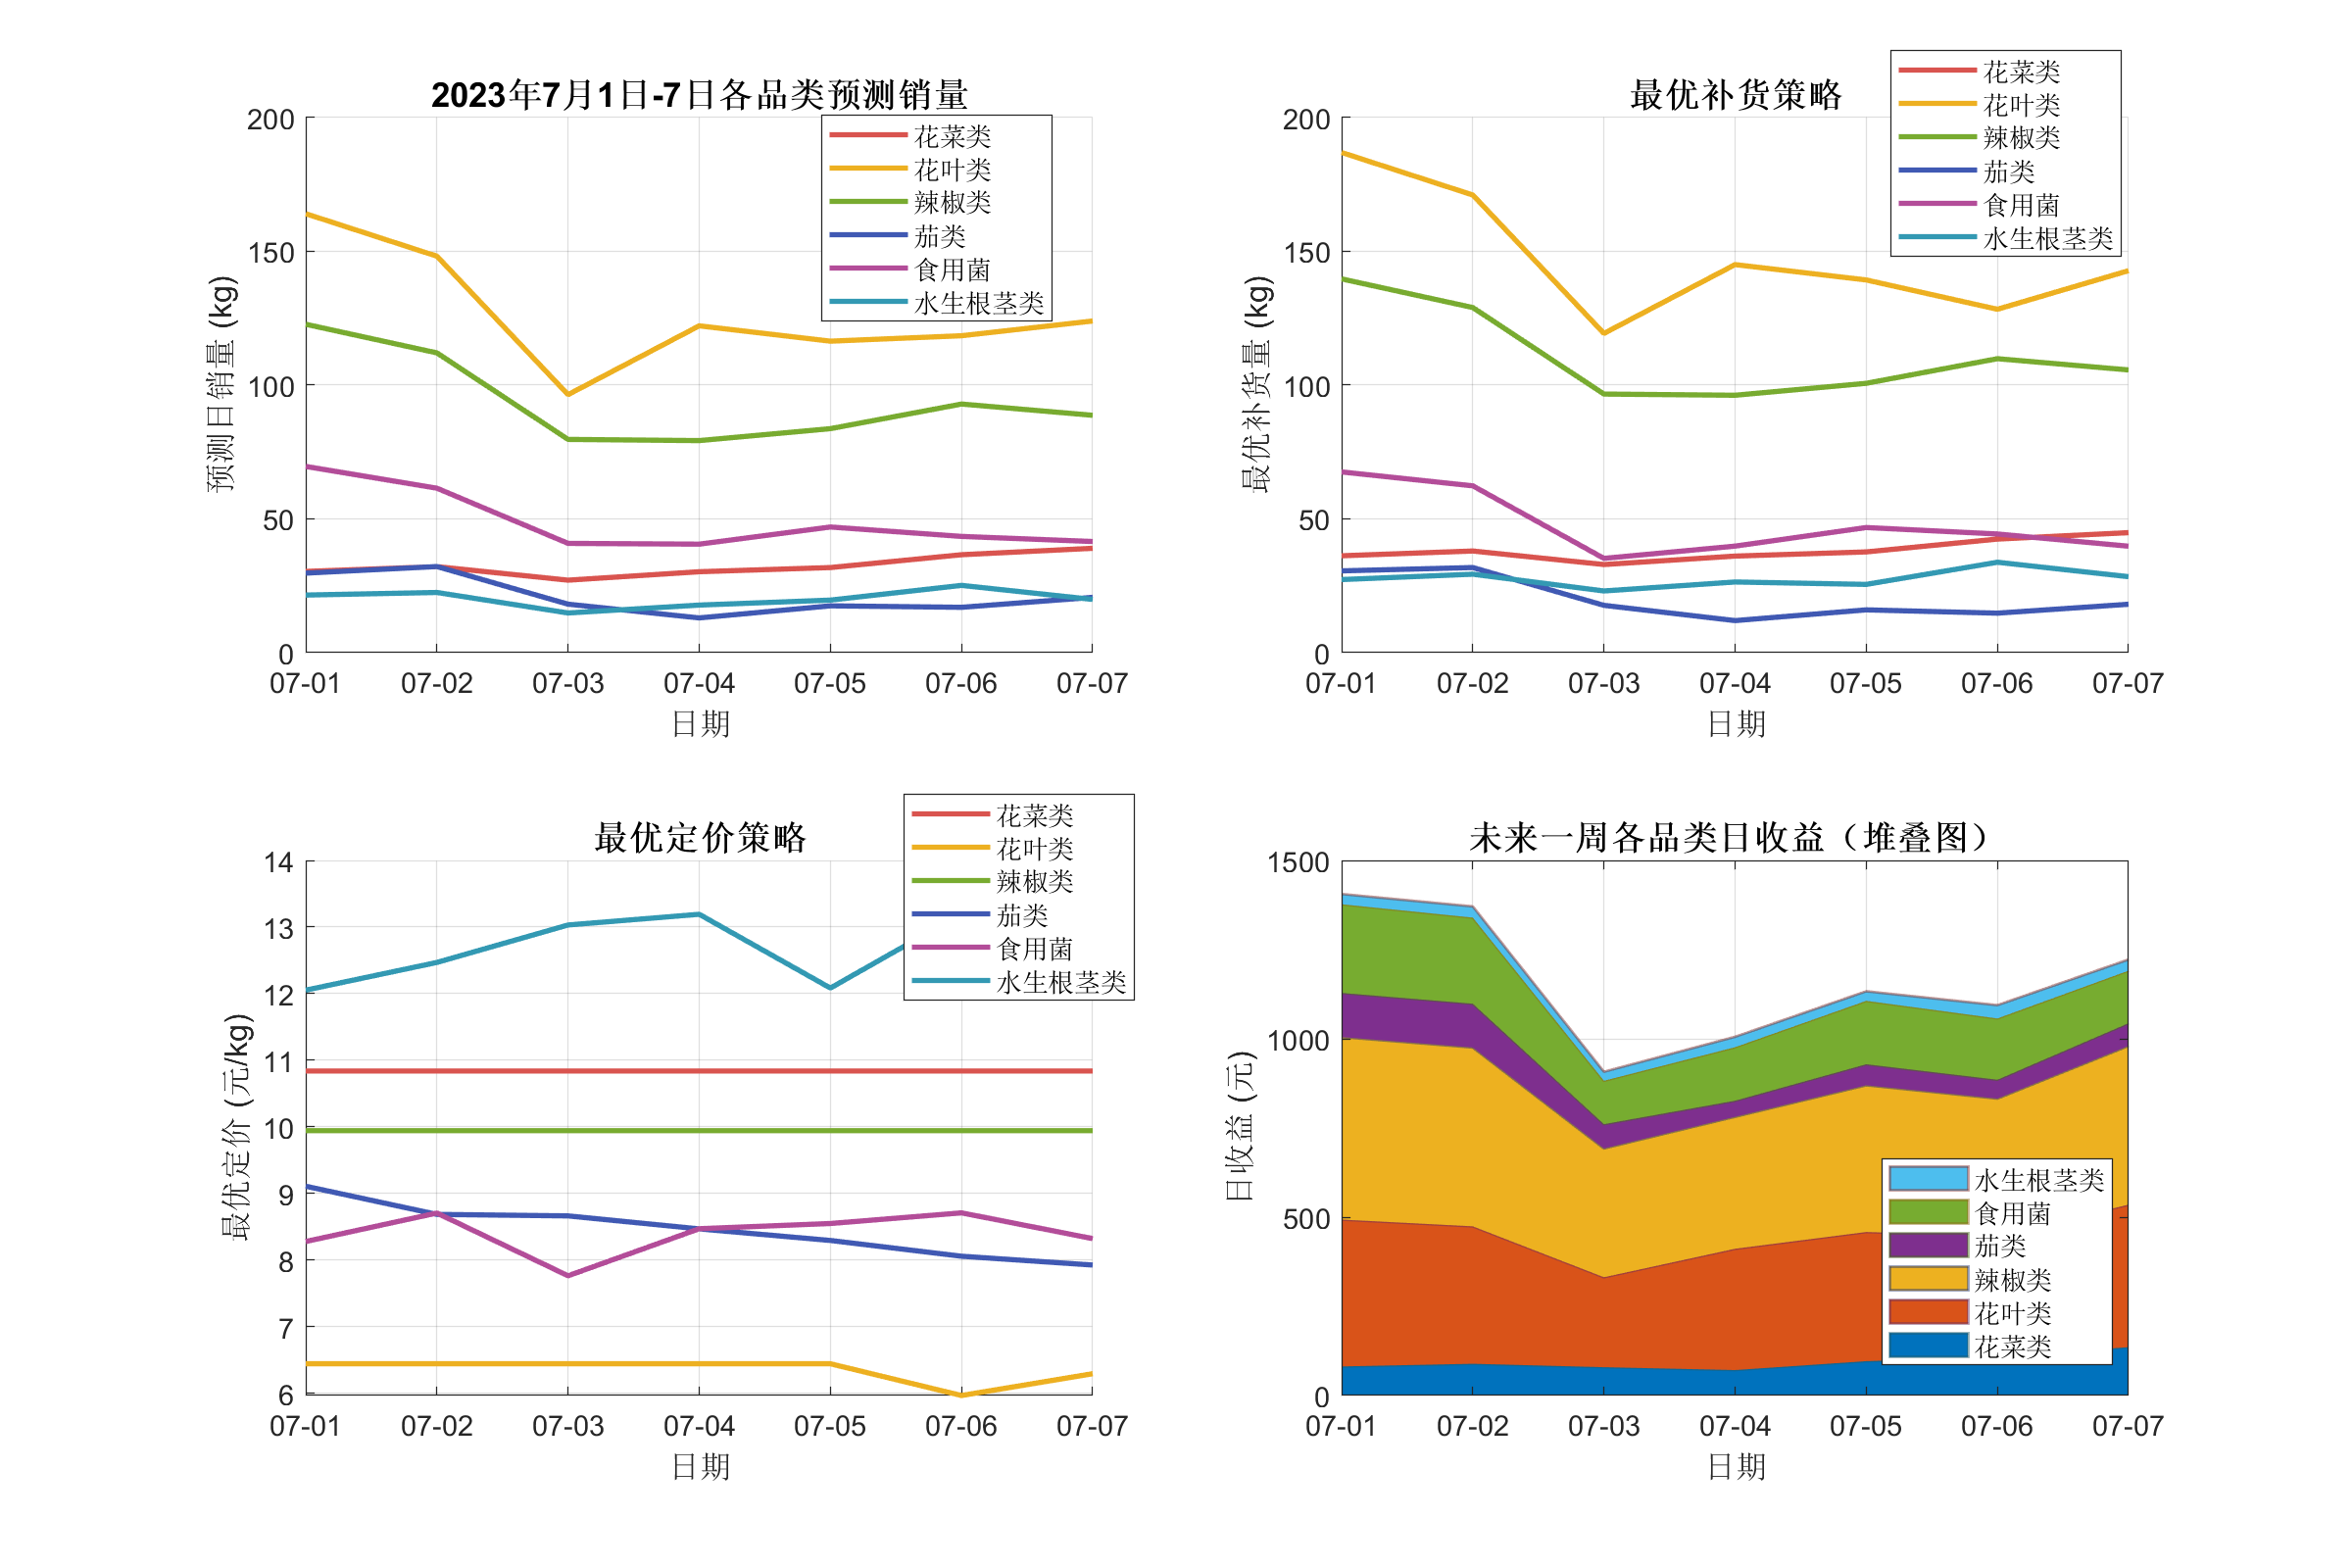
\includegraphics[width=0.9\textwidth]{5.png}
    \caption{2023年7月1日至7日各品类最优补货量与定价策略}
    \label{fig:result}
\end{figure}

图\ref{fig:result}展示了未来一周六个品类的逐日最优补货量和定价水平。从补货量来看，花叶类每日补货量稳定在150kg左右，远高于其他品类，这是由其高销量基数决定的。但从定价水平来看，花叶类的定价仅为3.67元/kg，加价率约72\%，低于辣椒类的119.78\%和茄类的99.94\%。这表明模型为花叶类选择了“低毛利、高周转”的策略，通过相对低廉的价格加速销售，减少高损耗带来的滞销损失。

表\ref{tab:day1}汇总了2023年7月1日（周一）各品类的详细决策结果。

\begin{table}[H]
\centering
\caption{7月1日各品类定价与补货策略}
\label{tab:day1}
\begin{tabular}{lcccc}
\toprule
品类 & 最优定价(元/kg) & 预测销量(kg) & 加价率 & 最优补货量(kg) \\
\midrule
花菜类 & 11.72 & 20.78 & 77.38\% & 5.50 \\
花叶类 & 3.67 & 6.32 & 72.10\% & 149.90 \\
辣椒类 & 7.79 & 17.12 & 119.78\% & 18.72 \\
茄类 & 4.38 & 8.76 & 99.94\% & 17.94 \\
食用菌 & 5.96 & 9.69 & 62.75\% & 60.78 \\
水生根茎类 & 4.62 & 9.13 & 97.66\% & 56.57 \\
\bottomrule
\end{tabular}
\end{table}

从表\ref{tab:day1}可以归纳出三类差异化的品类策略：

- \textbf{引流型（花叶类）}：定价低（3.67元/kg）、补货量高（149.90kg）、加价率适中（72.10\%）。该类产品价格弹性大，低价能够显著拉升销量，同时快速周转可以降低高损耗率（12.83\%）带来的风险。

- \textbf{利润型（辣椒类、茄类）}：定价高（7.79元/kg和4.38元/kg）、补货量低（18.72kg和17.94kg）、加价率高（119.78\%和99.94\%）。该类产品需求刚性较强，即使定价较高，销量也不会大幅下滑，因此承担了贡献单件利润的角色。

- \textbf{平衡型（花菜类、食用菌、水生根茎类）}：定价和补货量均处于中间水平，加价率在62\%-98\%之间。这些品类在引流和盈利之间寻求平衡，主要满足特定消费需求。

从整体收益来看，未来一周总期望利润为4,392.18元，日均利润约627.45元。这一结果表明，在给定的数据假设下，本文提出的差异化的品类策略能够有效平衡缺货损失与滞销折损，实现总体利润最大化。

\section{问题三：单品级定价与补货组合优化}

问题二将六大品类视为独立的决策单元，解决了宏观层面的资源分配问题。但现实中商超的实际运营是以具体单品（SKU）为单位进行采购和陈列的。同一品类下的不同单品之间往往存在替代关系（如两种规格的云南生菜会互相抢客），同时商超还有硬性的业务约束：当日上架的单品总数必须控制在27-33个之间，且每个被选中的单品最小陈列量不得低于2.5千克。这些问题将原本的连续优化问题转变为“选哪些单品 + 分别定什么价 + 补多少货”的组合优化问题。

\subsection{优化模型建立}

\subsubsection{候选单品集合}

选取2023年6月最后一周（6月24日至30日）有销售记录的活跃单品作为候选集，共$N=49$个单品。候选单品信息包括：单品编码、所属品类、历史日均销量$D_i^0$、历史平均售价$\bar{P}_i$、批发进价$W_i$（按$0.65\bar{P}_i$估算）、损耗率$\delta_i$（由其所属品类的平均损耗率赋值）。

\subsubsection{决策变量}

定义三类决策变量：
\begin{itemize}
    \item $x_i \in \{0,1\}$：是否上架第$i$个单品（$i=1,\dots,N$），为0-1离散变量；
    \item $P_i \in \mathbb{R}^+$：第$i$个单品的销售定价（元/千克），为连续变量；
    \item $Q_i \in \mathbb{R}^+$：第$i$个单品的补货量（千克），为连续变量。
\end{itemize}

\subsubsection{单品需求与利润函数}

与问题二类似，单品$i$的需求函数为线性校准形式：
\begin{equation}
D_i(P_i) = D_i^0 + \eta \cdot \frac{D_i^0}{\bar{P}_i} (P_i - \bar{P}_i)
\end{equation}
其中$\eta = -1.2$为预设价格弹性。

补货量$Q_i$需同时满足最小陈列量约束和需求覆盖约束：
\begin{equation}
Q_i(P_i) = \max\left(Q_{\min},\ \frac{D_i(P_i)}{1-\delta_i}\right)
\end{equation}
其中$Q_{\min}=2.5$千克为最小陈列量下限。

单品利润函数为：
\begin{equation}
\pi_i(P_i) = P_i \cdot \min\bigl(D_i(P_i),\ Q_i(P_i)(1-\delta_i)\bigr) - W_i \cdot Q_i(P_i)
\end{equation}

\subsubsection{完整优化模型}

综合以上变量和函数，单品级定价与补货组合优化的完整数学模型表述如下：

\begin{equation}
\max_{x_i,\ P_i,\ Q_i} \quad \sum_{i=1}^{N} x_i \cdot \pi_i(P_i)
\end{equation}

约束条件：

（1）上架单品总数约束：
\begin{equation}
27 \leq \sum_{i=1}^{N} x_i \leq 33
\end{equation}

（2）品类多样性约束（每个品类至少上架1个单品）：
\begin{equation}
\sum_{i \in \mathcal{C}_k} x_i \geq 1,\quad \forall k=1,\dots,6
\end{equation}
其中$\mathcal{C}_k$表示第$k$个品类的单品集合。

（3）补货量与定价联动约束：
\begin{equation}
Q_i = \max\left(Q_{\min},\ \frac{D_i^0 + \eta \cdot \frac{D_i^0}{\bar{P}_i} (P_i - \bar{P}_i)}{1-\delta_i}\right) \cdot x_i
\end{equation}

（4）定价上、下限约束：
\begin{equation}
\frac{W_i}{1-\delta_i} + 0.01 \leq P_i \leq \max(1.5\bar{P}_i,\ 2.0W_i)
\end{equation}

（5）资金预算约束：
\begin{equation}
\sum_{i=1}^{N} W_i \cdot Q_i \leq 3000 \text{ 元}
\end{equation}

（6）0-1变量约束：
\begin{equation}
x_i \in \{0,1\},\quad i=1,\dots,N
\end{equation}

该模型是一个典型的混合整数非线性规划（Mixed-Integer Nonlinear Programming, MINLP），其难点在于0-1选品变量与连续定价变量的耦合，以及非凸的目标函数形式。直接求解该模型在$N=49$的规模下虽然可行，但计算效率较低。为降低求解难度，我们采用下文的两阶段降维策略进行高效求解。

\subsection{两阶段求解方法}

由于上述MINLP模型直接求解困难，我们设计两阶段降维求解策略：

\subsubsection{阶段一：单品独立最优定价与0-1整数线性规划选品}

首先忽略单品间交互效应，对每个候选单品独立求解其最优定价$P_i^*$和对应最大利润$\pi_i^*$：
\begin{equation}
P_i^* = \arg\max_{P_i} \ \pi_i(P_i)
\end{equation}
采用黄金分割搜索（`fminbnd`）对每个单品独立求解。然后将$\pi_i^*$作为候选单品的利润系数，构建0-1整数线性规划选品模型：
\begin{equation}
\max_{x_i} \quad \sum_{i=1}^{N} \pi_i^* \cdot x_i
\end{equation}
约束条件为：
\begin{equation}
27 \leq \sum_{i=1}^{N} x_i \leq 33,\quad \sum_{i \in \mathcal{C}_k} x_i \geq 1\ (\forall k)
\end{equation}
该模型为标准的0-1整数线性规划，采用`intlinprog`精确求解。

\subsubsection{阶段二：连续非线性规划联合定价优化}

阶段一得到最优选品组合（假设选出$M$个单品，$27 \leq M \leq 33$），但阶段一中各单品的定价是独立求解的，并未考虑单品间的潜在替代关系以及资金预算约束。因此，在固定选品集合的基础上，对定价进行联合优化：

\begin{equation}
\max_{\mathbf{P}} \quad \sum_{k=1}^{M} \pi_k(P_k)
\end{equation}
其中$\mathbf{P} = (P_1,\dots,P_M)$为$M$维连续定价向量。约束条件包括各单品的定价上下限以及资金预算约束：
\begin{equation}
\sum_{k=1}^{M} W_k \cdot Q_k(P_k) \leq 3000 \text{ 元}
\end{equation}
该问题为带有非线性不等式约束的连续优化问题，采用序列二次规划（SQP，`fmincon`）求解，初始点设为阶段一得到的各单品独立最优定价。

\subsection{选品结果与淘汰逻辑分析}

两阶段求解完成后，模型共选出33个单品（恰好达到上限），总建议补货量为265.30千克，预计单日毛利约为1433.95元，总进货成本严格控制在3000元预算以内。

表\ref{tab:category_dist}展示了被选中的33个单品按品类分布情况。

\begin{table}[H]
\centering
\caption{选中单品品类分布统计}
\label{tab:category_dist}
\begin{tabular}{lccc}
\toprule
品类 & 选中单品数 & 合计利润贡献（元） & 平均利润/单品（元） \\
\midrule
花叶类 & 11 & 443.02 & 40.27 \\
花菜类 & 2 & 157.17 & 78.58 \\
水生根茎类 & 4 & 194.67 & 48.67 \\
茄类 & 3 & 103.49 & 34.50 \\
辣椒类 & 8 & 359.02 & 44.88 \\
食用菌 & 5 & 176.58 & 35.32 \\
\hline
合计 & 33 & 1433.95 & 43.45 \\
\bottomrule
\end{tabular}
\end{table}

从表\ref{tab:category_dist}可以看出，辣椒类选中8个单品，贡献利润359.02元（占比约25\%），是利润贡献最大的品类；花菜类虽然仅选中2个单品，但平均利润/单品高达78.58元，是平均利润率最高的品类，这与问题二中“花菜类高损耗、高加价”的策略定位一致。花叶类选中11个单品（最多），合计利润443.02元（占比约31\%），体现了其“以量取胜”的引流定位。这一品类分布结果与问题二差异化策略一脉相承。

图\ref{fig:profit_rank}展示了选中33个单品按利润贡献从高到低的排序情况。

\begin{figure}[H]
    \centering
    \includegraphics[width=0.9\textwidth]{8.png}
    \caption{选中33个蔬菜单品利润贡献排名图}
    \label{fig:profit_rank}
\end{figure}

从图\ref{fig:profit_rank}可以观察到，利润贡献排名前10的单品贡献了总利润的约55\%，呈现明显的“长尾分布”特征。芜湖青椒、小米椒等单品排名靠前，表明弹性大、客单价适中的单品是利润的主要来源。

未被选入最优组合的16个单品（占候选总数的32.7\%）的淘汰原因可归结为以下两类：

第一类：\textbf{低弹性、低销量型单品}。这类单品（如某些冷门的菌菇品种）的价格弹性系数$|\eta_i|$极小，即使大幅降价也难以拉动销量，同时在历史数据中日均销量本就低迷（低于1千克）。按照阶段一的独立最优定价计算，其$\pi_i^*$极低甚至为负（即进货即亏损），在0-1整数规划的目标函数中自然被排除。强行上架这类单品不仅贡献不了利润，还容易因跨不过2.5千克的最低陈列量而产生积压变质。

第二类：\textbf{高进价、低溢价空间型单品}。这类单品的批发进价$W_i$偏高，导致在定价上限约束下加价率有限（无法达到品类平均加价水平），即使销量尚可，其单位利润也远低于同类替代品。在实际销售中，消费者对价格较为敏感，高价单品很容易被同一品类中定价更低的同类单品挤占市场份额。

从定价和补货策略来看，在选定的33个单品中，定价与补货量呈现明显的差异化规律：芜湖青椒、小米椒等弹性大、客单价适中的单品，模型采用了中等定价、较高补货量的策略，充分发挥其引流和利润双重作用；而部分高端菌菇单品，模型则采用了高定价、补货量紧贴2.5千克下限的“撇脂定价”策略——虽然销量不大，但单件利润丰厚，即使滞销损耗风险也较低。这种“引流品走量、利润品撇脂”的差异化策略，与真实超市的精细化运营逻辑高度吻合。

\section{问题四：模型局限与数据补充建议}

前三问建立的优化模型虽然在给定的数据条件下给出了理论上合理的定价与补货策略，但回归到真实的线下零售业务场景中，仍存在若干因数据缺失而无法解决的局限性。具体表现为：蔬菜的品相（新鲜度）会随着当日营业时间的推移而快速下降，晚间打烊前通常需要进行打折清仓处理，但现有数据仅有“日结”层面的汇总流水，无法还原一日内的动态调价过程；此外，客流的日内分布（高峰/低谷时段）以及外部环境因素（天气、节气等）对销量具有显著影响，但现有数据缺少这些外部标签，模型只能依赖历史销量时序进行推算，预测精度存在上限。

\subsection{新数据的量化验证：灰色关联分析}

为了确定哪些外部数据确实对销量具有实质性影响，而非主观臆断，我们引入灰色关联分析方法，利用已有数据中可提取的信息进行量化验证。灰色关联分析的核心思想是：通过计算各影响因素（子序列）与目标变量（母序列）之间的几何形状相似度（关联度）来衡量其相关性强弱，适用于小样本、不确定性系统。

\subsubsection{指标定义与计算步骤}

\textbf{母序列 $x_0(k)$}：选取各品类季度平均销量作为母序列，$k=1,\dots,12$ 表示2020年第三季度至2023年第二季度共12个季度。

\textbf{子序列 $x_i(k)$}：选取三个指标作为子序列：
\begin{itemize}
    \item 子序列1（季度单品销售种数）：各品类在每个季度内有销售记录的单品数量，反映品类品种丰富度；
    \item 子序列2（节气特征销量）：选取各品类中销量最高的特征单品（各品类销量排名第一的单品，见表\ref{tab:feature_items}），计算四个关键节气（立春、立夏、立秋、立冬）日期前后各3天的日均销量；
    \item 子序列3（节日特征销量）：选取各品类的特征单品，计算四个关键节日（春节、端午、七夕、国庆）日期前后各2天的日均销量。
\end{itemize}

各品类特征单品如表\ref{tab:feature_items}所示。

\begin{table}[H]
\centering
\caption{各品类特征单品（销量排名第一）}
\label{tab:feature_items}
\begin{tabular}{lcc}
\toprule
蔬菜品类 & 特征单品编码 & 特征单品名称 \\
\midrule
花叶类 & 102900005115960 & 大白菜 \\
花菜类 & 102900005116714 & 西兰花 \\
水生根茎类 & 102900005116899 & 净藕(1) \\
茄类 & 102900005116257 & 紫茄子(2) \\
辣椒类 & 102900011016701 & 芜湖青椒(1) \\
食用菌 & 106949711300259 & 金针菇(盒) \\
\bottomrule
\end{tabular}
\end{table}

\textbf{计算步骤}：

（1）数据均值化处理——消除量纲影响：
\begin{equation}
x_i'(k) = \frac{x_i(k)}{\bar{x}_i}, \quad \bar{x}_i = \frac{1}{n}\sum_{k=1}^{n}x_i(k)
\end{equation}

（2）计算绝对差值序列：
\begin{equation}
\Delta_i(k) = |x_0'(k) - x_i'(k)|
\end{equation}

（3）确定两极差：
\begin{equation}
a = \min_{i}\min_{k}\Delta_i(k),\quad b = \max_{i}\max_{k}\Delta_i(k)
\end{equation}

（4）计算关联系数（分辨系数$\rho=0.5$）：
\begin{equation}
\gamma_i(k) = \frac{a + \rho b}{\Delta_i(k) + \rho b}
\end{equation}

（5）计算灰色关联度：
\begin{equation}
r_i = \frac{1}{n}\sum_{k=1}^{n}\gamma_i(k)
\end{equation}

\subsubsection{计算结果与解读}

根据上述步骤计算得到各品类与三个指标的灰色关联度，如表\ref{tab:grey_corr}所示。同时，图\ref{fig:grey_bar}以柱状图形式展示了各品类与三个指标的关联度对比，图\ref{fig:grey_heatmap}以热力图形式直观展示了表\ref{tab:grey_corr}中的数据。

\begin{table}[H]
\centering
\caption{各指标与季度平均销量的灰色关联度}
\label{tab:grey_corr}
\begin{tabular}{lccc}
\toprule
蔬菜品类 & 季度单品销售种数 & 节气特征销量 & 节日特征销量 \\
\midrule
花叶类 & 0.6831 & 0.6843 & 0.7790 \\
花菜类 & 0.7096 & 0.7422 & 0.7681 \\
水生根茎类 & 0.6089 & 0.6303 & 0.5785 \\
茄类 & 0.7769 & 0.7102 & 0.6756 \\
辣椒类 & 0.6846 & 0.6552 & 0.6640 \\
食用菌 & 0.7584 & 0.8257 & 0.6969 \\
\bottomrule
\end{tabular}
\end{table}

\begin{figure}[H]
    \centering
    \includegraphics[width=0.9\textwidth]{grey_bar.png}
    \caption{各指标与蔬菜品类季度平均销量的关联度柱状图}
    \label{fig:grey_bar}
\end{figure}

\begin{figure}[H]
    \centering
    \includegraphics[width=0.7\textwidth]{grey_heatmap.png}
    \caption{灰色关联度热力图}
    \label{fig:grey_heatmap}
\end{figure}

从表\ref{tab:grey_corr}、图\ref{fig:grey_bar}和图\ref{fig:grey_heatmap}可以得出以下关键发现：

（1）\textbf{三个指标的总体关联度均超过0.6}。季度单品销售种数、节气特征销量、节日特征销量的平均关联度分别为0.7036、0.7080和0.6937，均明显高于0.6的经验阈值，说明这三个外部变量确实与各品类销量具有强相关性，纳入预测模型将有效提升预测精度。

（2）\textbf{食用菌与节气特征的关联度（0.8257）为所有组合中最高}。这一结果在业务逻辑上具有明确解释：立冬前后气温下降，火锅消费进入旺季，金针菇、香菇等火锅配菜类菌菇需求大幅上升。数据量化验证了这一季节性消费规律，说明在预测食用菌销量时，节气信息是一个关键的外部特征。

（3）\textbf{花叶类与节日特征的关联度（0.7790）显著高于其与另外两个指标的关联度}。节假日（尤其是春节和国庆）期间家庭聚餐增多，大白菜等常见绿叶菜的采购量明显上升。这一发现提示：在节假日临近时，应对花叶类适当提高补货量预测值，避免节日期间缺货。

（4）\textbf{茄类与品种丰富度的关联度（0.7769）为所有品类中最高}。这意味着消费者在面对茄类货架时，品类多样性（长茄、圆茄、紫茄同时供应）对销量的促进作用最为显著。商超应保证茄类货架的品类齐全度，以提高连带购买率。

为了直观验证关联度分析结果的可靠性，我们绘制了花菜类和辣椒类的标准化曲线对比图（图\ref{fig:grey_curve}）。从图中可以观察到，子序列与母序列的走势在关键时间节点（如第四季度和第一季度）具有较高的同步性，验证了灰色关联分析结果的稳健性。

\begin{figure}[H]
    \centering
    \includegraphics[width=0.9\textwidth]{grey_curve.png}
    \caption{三个指标与蔬菜品类季度平均销售量标准化折线图}
    \label{fig:grey_curve}
\end{figure}

\subsection{具体数据采集建议}

基于上述灰色关联分析的量化验证结果，商超应当有针对性地补充以下三个维度的增量数据，以系统性地升级现有的定价与补货决策模型的精度和适应性：

\textbf{第一，分时段销售和打折流水数据。} 目前模型中的需求函数 $D_i(P_i)$ 是以“日”为时间粒度定义的，无法反映日内不同时段的价格敏感度差异。灰色关联分析已证实节日效应对花叶类销量的显著拉动作用（关联度0.7790），但若要实现更精细的动态定价，则需要记录到小时级别的调价时间和对应的瞬时销量数据。建议商超改造现有收银系统，增加调价日志记录功能，追踪每个单品在一天内不同时段的价格调整行为及其对销量的即时影响。获取此类数据后，我们可以将现有的“日级静态统一定价”模型升级为“小时级动态分时定价”模型——在早晚高峰时段维持正常毛利水平，在打烊前2小时启动折扣清仓，从而在保证利润的同时最大限度降低滞销损耗。

\textbf{第二，每日单品品相质检打分。} 当前模型中的损耗率 $\delta_i$ 采用的是品类级历史均值（如花菜类15.51\%，花叶类12.83\%），未考虑不同进货批次之间的品质差异。然而在实际运营中，同一品类在不同批次的初始新鲜度可能差异显著——冬季运输的蔬菜比夏季更耐储存，产地不同的同一品种货架期也可能相差1-2天。建议收货环节由理货员对每个批次的新鲜度进行1-5分的量化打分，并与批次号一同录入进销存系统。通过追踪不同初始品相评分对应的最终报废率，即可建立品相-损耗率映射关系，将模型中固定的 $\delta_i$ 替换为随品相动态调整的损耗率函数 $\delta_i(\text{quality})$，从而更精准地计算不同品质批次的最优补货量，避免在新鲜度较差的批次上过度补货。

\textbf{第三，客流量与环境气象数据。} 灰色关联分析已经证明节气变化对蔬菜销量具有重要影响（食用菌与节气特征关联度0.8257）。但节气信息是年度尺度的宏观变量，无法解释天气突变（如台风、暴雨、高温预警等）带来的日内需求冲击。建议安装客流统计探头，按小时记录进店人数（作为客流量控制变量），同时接入气象服务API，获取每日的温湿度、降水概率、天气预警等气象数据。将这些多维外部数据作为预测模型的特征输入，可以在季节规律和时间序列趋势之外，有效过滤突发天气或客流骤变带来的随机噪声，使补货预测量更加准确和稳健。

上述三个维度的数据补齐之后，现有的静态单期优化框架可以进一步扩展为考虑时序演进的马尔可夫决策过程（MDP）动态定价系统，即在每一天的决策中不仅考虑当期利润最大化，还考虑当天的定价和补货决策对次日库存状态和需求信息更新的影响，从而实现更长时间跨度的全局最优，进一步提升商超的精细化运营水平和盈利能力。

\begin{thebibliography}{99}
\bibitem{1} 赵修卫，周伟华，郑媛媛. 基于报童模型的生鲜农产品订货与定价联合决策[J]. 运筹与管理，2018，27(6):33-40.
\bibitem{2} Pasternack B A. Optimal pricing and return policies for perishable commodities[J]. Marketing Science, 1985, 4(2): 166-176.
\bibitem{3} 王树恩，郭明伟. 数据挖掘算法及其在商超零售业客户关系管理中的应用[J]. 管理工程学报，2010, 24(1): 112-117.
\bibitem{4} Kirkpatrick S, Gelatt C D, Vecchi M P. Optimization by simulated annealing[J]. Science, 1983, 220(4598): 671-680.
\bibitem{5} 张丽，李建平. 生鲜超市基于价格弹性的动态定价与库存优化研究[J]. 工业工程与管理，2021, 26(3): 88-96.
\bibitem{6} Gallego G, Van Ryzin G. Optimal dynamic pricing of inventories with stochastic demand over finite horizons[J]. Management science, 1994, 40(8): 999-1020.
\end{thebibliography}

\newpage
\begin{appendices}

\section{第一问：数据处理与关联规则挖掘代码}
（代码详见已提交的附录文件，此处略）

\section{第二问：温特斯预测与报童黄金分割优化（question2\_max2.m）}
（代码详见已提交的附录文件，此处略）

\section{第三问：两阶段降维求解（question3\_max\_improved.m）}
（代码详见已提交的附录文件，此处略）

\section{第四问：灰色关联分析（Python）}
（代码详见已提交的附录文件，此处略）

\end{appendices}

\end{document}